% hello.tex - our first latex example

\documentclass[a4paper]{report}
\usepackage{titlesec}
\usepackage{graphicx}
\usepackage{framed}
\usepackage{pdfpages}
\usepackage{wrapfig}

\addtolength{\oddsidemargin}{-.5in}
\addtolength{\evensidemargin}{-.5in}
\addtolength{\textwidth}{1in}


\title{MOS : A Multitasking Operating System}
\date{\today}
\author{Michael Rochester\\ Candidate: 23344\\ University of Sussex
        \and Supervisor:\\ Martin Berger}


\setcounter{tocdepth}{4}
\setcounter{secnumdepth}{4}
\begin{document}

\titlespacing*{\chapter}{0pt}{-50pt}{20pt}
\titleformat{\chapter}[display]{\normalfont\huge\bfseries}{\chaptertitlename\ \thechapter}{20pt}{\Huge}


\maketitle

\tableofcontents
\listoffigures

\chapter{Introduction}

The overall aim for this project is to produce a simple Multitasking Operating System (herein called MOS), following 5 key tenants, to study structure, allocation, and management of different classes of resource. This section provides a brief introduction to Operating Systems, Discusses the project aims, and looks at the approach take.

We live in a world surrounded and controlled by machines, and software is our way of telling those machines how to act. As our machines and needs become more complex, so must the software that runs them. An Operating System is a software package that allows for others to easily create complex behaviours by providing simple high level abstractions over the intricate low level hardware.









\clearpage
\section{Understanding Operating Systems}


Before this project can even begin, an understanding of what a Operating System is and does is required.

Operating Systems come in all different shapes and sizes, however usually they contain three distinct parts:

The kernel is the software that drives the hardware. It provides nice abstractions and interfaces to control the very fiddly underlying machine.

The Bootloader is the code that is run first. It gets things that the kernel might need set up, for example, getting the CPU into the correct operation mode.

The Final part is a collection of programs and other software that come with the Operating System. Although some people would argue this is not so much part of the Operating System, on some systems (namely Microsoft's Windows) a huge number of these programs are built right in, and seem from the outside to be part of the kernel.

\subsection{The Bootloader}

\begin{figure}[ht]
\centering
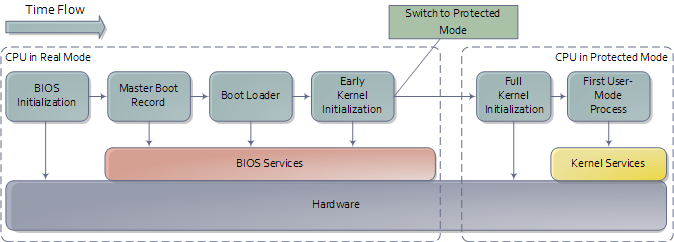
\includegraphics[width=415px]{images/bootProcess.png}
\caption{An Example of a boot cycle. The bootloader is in control while the CPU is in Real Mode.}
\label{fig:theloader}
\end{figure}

The bootloader's job is to load the kernel. First off, the CPU has to begin executing code somewhere, most of the time this is done by the BIOS, which detects our bootloader and starts it running.

The majority of the rest of the bootloader's job is to get the hardware ready for the kernel to take over. Tasks like detecting the available physical memory of a machine is up to the bootloader, once it has gathered such information, the loader will store it somewhere the kernel can find it.

The final steps of the bootloader are to get the CPU into the right mode. It does this by first setting up some important `tables' in memory. One of these tells the CPU what to do if an interrupt is produced. Another tells the CPU where it can find physical addresses in RAM when virtual addresses are looked up.

Finally the bootloader can jump to the start of the kernel and it's job is finished.

\clearpage
\subsection{The Kernel}

\begin{wrapfigure}{r}{150px}
\centering
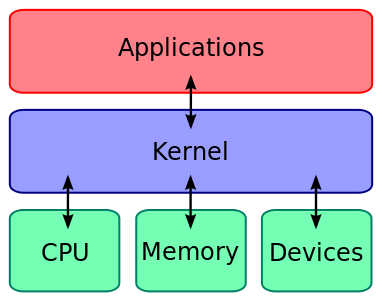
\includegraphics[width=150px]{images/kernel}
\caption{The Kernels Role is to make using the hardware easier for programs.}
\vspace{-10pt}
\label{fig:thekernel}
\end{wrapfigure}

Once the bootloader has passed control to the kernel, the kernel begins to prepare for executing programs. It will create tables of information, most of which will be empty to begin with, but they will quickly be filled. Some of the more important tasks are keeping track of which processes are currently executing and deciding which should go next, as well as ensuring that all processes think they have enough memory to operate correctly.

Once the kernel is happy that everything is in order, it will begin execution of the first process. For the rest of the time the computer is on, `processes' will be run. These processes are pieces of code that perform some form of task, each having a unique environment. As far as a process is concerned, it owns the whole computer. However, as programmers are aware that each process does not own the whole computer, they can program complex interprocess interactions, with the kernels help of course.


\subsection{The Built in Programs}

\begin{wrapfigure}{r}{250px}
\centering
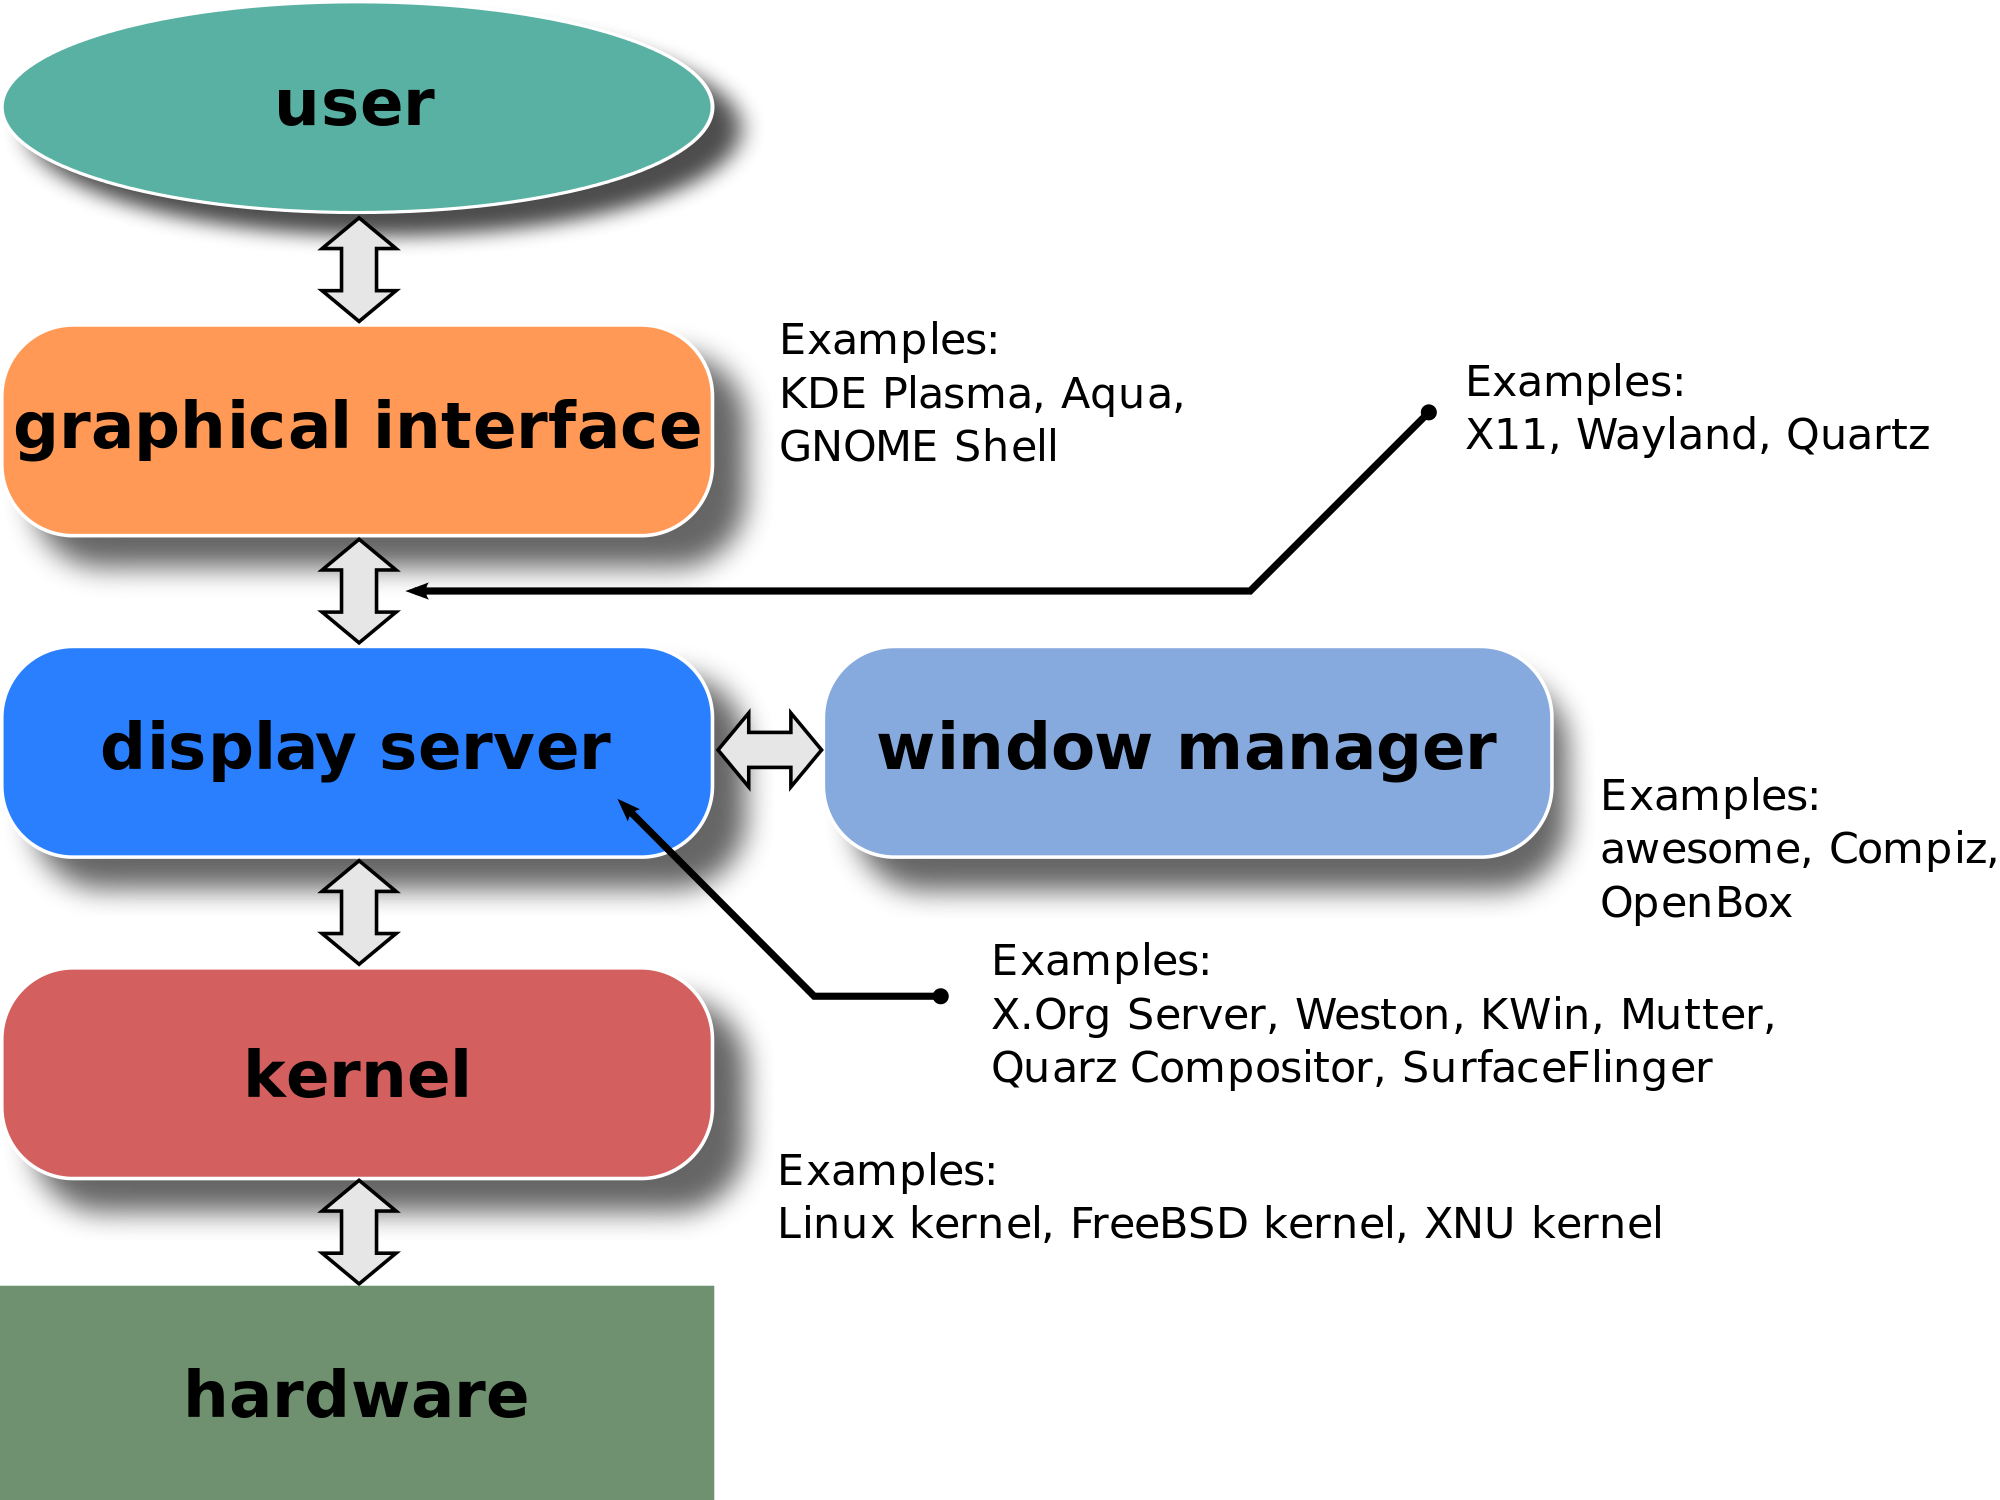
\includegraphics[width=250px]{images/windowing}
\caption{An example windowing server architecture.}
\label{fig:theserver}
\end{wrapfigure}

After the kernel starts process 0, process 0 is free to spawn many other programs. Many of these programs will come `built in' to an Operating System to create a richer platform for users.

Some would argue that these programs are not part of the Operating System its self. For example, in the Linux terminology, a kernel plus a collection of programs is referred to as a `Distro' or distribution of Linux. In Windows however, many of these programs are well integrated into the kernel and are considered part of the Operating System.

Figure \ref{fig:theserver} shows how even showing simple windows on the screen requires many levels of different programs interacting with each other. This architecture is favored amongst some computer users as it is more flexible and customizable to their own needs.
















\clearpage
\section {Project Aims}

The project was begun with a number of Primary and Extended Objectives, however as the project progressed, new objectives were discovered. These new objectives were prioritised over other extended objectives. This lead to some of the original extended objectives being left incomplete.

\textbf {Primary Objectives:}

\begin{itemize}
\item Create a bootloader to boot a kernel.
\item Create a kernel that should be able to:
\begin{itemize}
\item Load multiple `programs' into memory.
\item Execute multiple `programs' pseudo simultaneously using time sliced scheduling.
\item Allow multiple `programs' asynchronous access to areas of the terminal screen.
\item Allow for the management of the execution state of each `program'.
\item Allow each `program' access to a unique memory space.
\item Allow `programms' to asynchronously send data to each other.
\item Handle all common cpu interrupts and resolve them correctly.
\item Handle keyboard input and allow programs to `collect' keyboard inputs.
\end{itemize}
\item Create a small set of `programs' with which to test the kernel.
\end{itemize}

\textbf {Extended Objectives:}


\begin{itemize}
\item \lbrack Complete\rbrack Add some hardware drivers to load programs off disk and have some persistence.
\item \lbrack Partially Complete \rbrack Implement the entire c standard library.
\item Move into pixel graphics mode.
\item Use Multiple core's to have `true' concurrency.
\item Port the `Python' runtime to my OS (here I have chosen Python simply because there is a well documented `todo' list for porting python to new OS's).
\end{itemize}

\textbf {New Objectives:}


\begin{itemize}
\item \lbrack Complete\rbrack Create A user manual.
\item \lbrack Complete\rbrack Create A Developers manual.
\item \lbrack Complete\rbrack Create set of scripts for getting the source code, Building the project, and deploying it to a computer.
\end{itemize}








\chapter{Professional Considerations}

As this project falls within the bound of Computer Science, It will comply with the British Society of Computing (BSC) Code of Conduct \cite{CoC}. Although there is no contractual obligation to follow this code, it is important to recognize and comply with them to ensure the integrity of the project.

Each of the four main sections of the Code of Conduct will be discussed in order;

\section{Public Interest}

For this project no user information is gathered and the project poses no risk to a users health, privacy, or well-being.

The project makes use of third party material, however only within the licenses set out by those third parties that have been implicitly agreed to by all project members. Furthermore, it is explicitly marked where third party technologies were used.


\section{Professional Competence and Integrity}

The project was created as an undergraduate Final Year Project for a computer science course. It pulls knowledge from many of the modules taught as part of this course.

During the completion of the project The project engineer, Michael Rochester, will meet with a supervisor to ensure that he maintains professional competence and considers ideas and viewpoints he may not have considered.

\section{Duty to Relevant Authority}

A structure of meetings, and other feedback channels have been established between the project engineer, Michael Rochester, and the supervisors to ensure he is working in accordance with the University of Sussex guidelines.

\section{Duty to the Profession}

The project engineer, Michael Rochester, will carry out this project to the highest standard possible to maintain the reputation of the profession, furthermore all materials produced as part of this project will be freely available to any member of the profession to help further the understanding of the project domain.

\section{Requirement for ethical review}

This Project is a technical exercise in understanding the low level relationship between hardware and software, due to this, the project does not require human participation, testing, or feedback. As such, The Project does not require an ethical review, and there are no ethical concerns with this project.

\clearpage
\chapter{Requirements Analysis}

In preparation of producing an Operating System, current generation systems were studied in detail. The features and interfaces of the systems were analysed to assist in the designing of the MOS. Although It was known in advanced that MOS was not going to be complex enough to incorporate all features of the reference systems, it was important to study what current systems do, such that their most important features could be mimicked.

Modern Operating Systems are such that there are two user groups.


The End Users are the people using the Operating System and its programs to assist in achieving an assortment of tasks. To them, the Operating System provides a few simple mechanisms to interact with the system, E.G. Launching programs, closing programs, and switching between the `focused' program. Most of the inner workings of the Operating System are hidden from the end user, and they mainly interact with the `User space programs', which are not defined by the Operating System Developer.


The Program Developers use an Operating System as a platform to create the programs the End User will use. To them, the Operating System is a Resource Manager and Scheduler and provides some crucial functionality for complex behaviours like creating new processes, Allocating dynamic memory, allocating screen space to the programs, and accesing the hard drive. Many of the complexities of the Operating System (especially hardware control) are abstracted away from the Program Developers, however it is expected that they have some awareness of how the system is structured to successfully integrate with the kernel.

\clearpage
\section{The End User}
The reference systems that were studied with the End Users in mind are: The Linux distribution remix `Gnomebuntu' and the Microsoft Operating System `Windows 8'. These systems were chosen to get a spread in our sample. The systems are both popular desktop systems, however: One, (Linux) is stemmed from an open source mentality, where the source code is freely available and the system is free, and the other (Windows) is produced by a company with the aim to provide paying business, and home customers with a usable system.

The parts of the reference systems that were analysed from the end users perspective are; program launching, process management, and program interaction as these are the main sections that will be implemented in the MOS.

\subsection{Launching programs in Linux and Windows}

In both reference systems, the `windows' key is used to expose the program launching interface.

In Windows, the interface is a customizable, horizontal-scrolling, tile-based launcher. Each tile can be set to launch an application, or even launch a sub-activity of certain applications. Furthermore each Tile can give basic information of the internal state of the programs, even when the program is not properly running. (see Figure \ref{fig:WinLaunchScreen}.)


In Linux, the interface is a alphabetized list (with icons) of installed programs, sorted into pages. Pages can be navigated with vertical scrolling, or by jumping directly to a page represented by dots to the right of the screen. Linux also provides a `quick launch bar' (on the left of the screen) that can be accessed by simple pushing your cursor to the left edge of the screen. This allows for quicker launching of your favorite programs (see Figure \ref{fig:LinLaunchScreen}.)


\begin{figure}[ht]
\centering
\begin{minipage}{.5\textwidth}
  \centering
  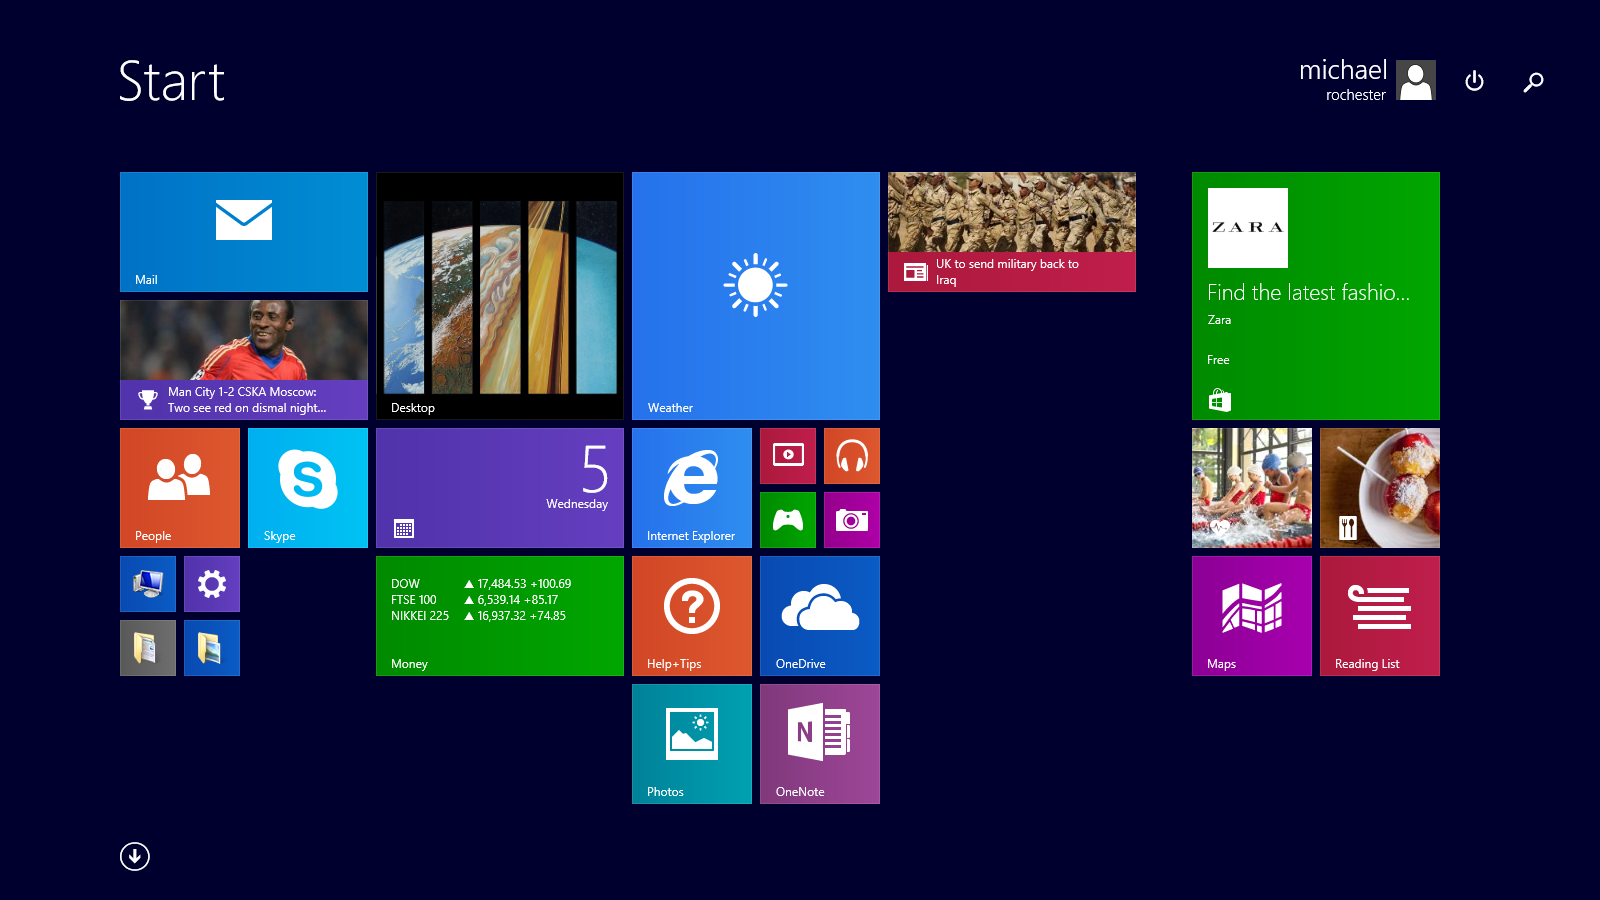
\includegraphics[width=200px]{images/Windows_Program_Launcher_Screenshot}
  \caption{Windows Program Launcher Interface}
  \label{fig:WinLaunchScreen}
\end{minipage}%
\begin{minipage}{.5\textwidth}
  \centering
  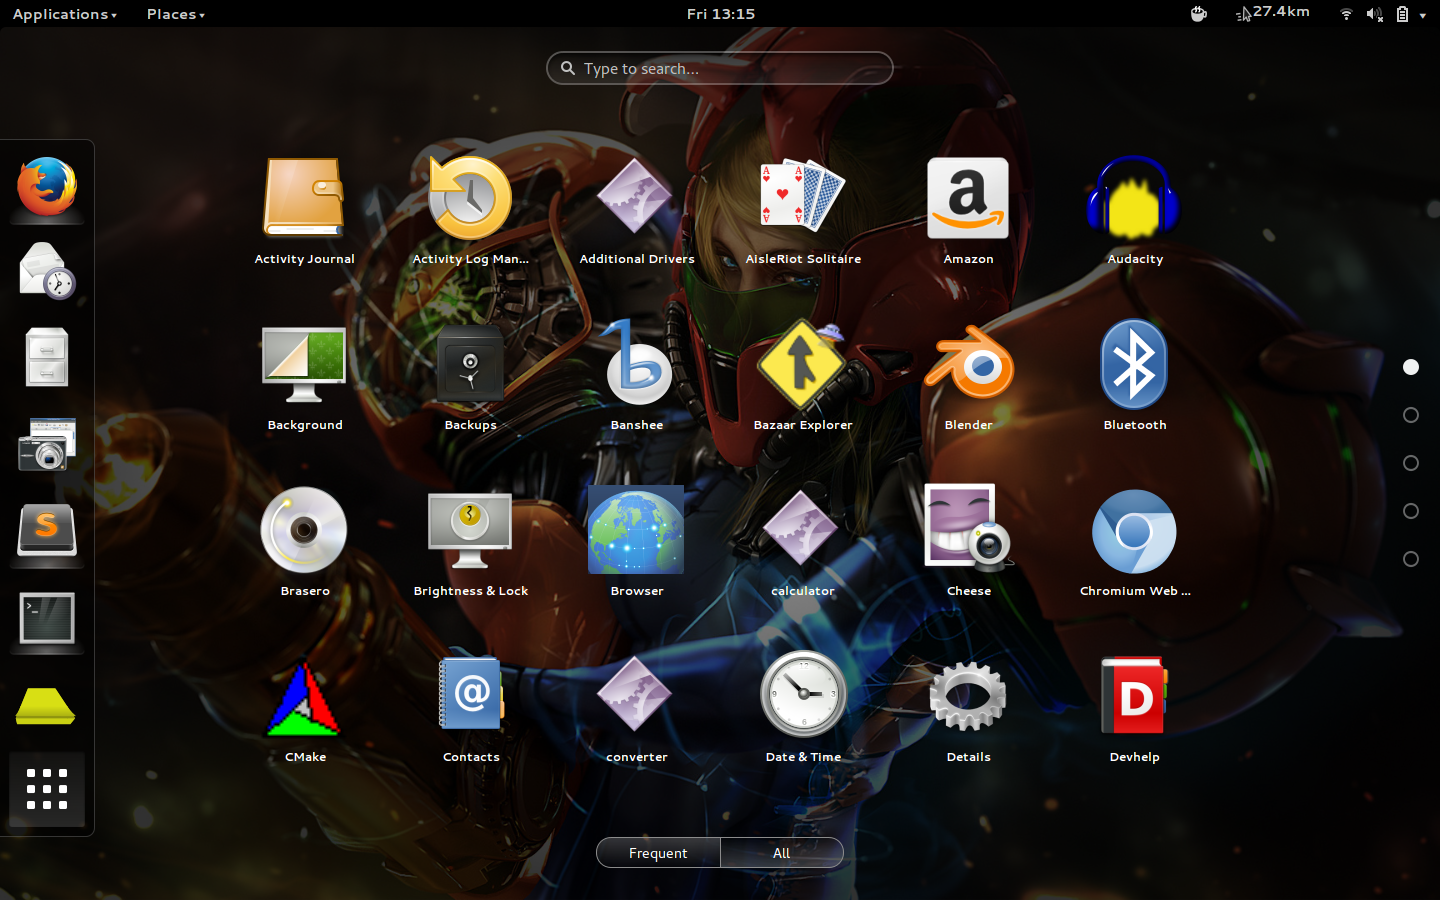
\includegraphics[width=200px]{images/Linux_Program_Launcher_Screenshot}
  \caption{Linux Program Launcher Interface}
  \label{fig:LinLaunchScreen}
\end{minipage}
\end{figure}


\subsection{Managing running programs in Linux and Windows}

Both reference systems provide a way of interacting directly with the process manager to give the user power over which programs are running on their system.

In each system, the process manager is very similar, as the tasks they perform are identical. Both systems provide a window that lists processes and some relevant information about each process like PID, cpu usage, memory usage, disk usage, and network usage. It was found that the majority of these fields are concerned with what resources a process is using. This is the case because an Operating System's purpose is to manage the physical resources available to the software.

Each system also provides the ability to change what information is provided for each process, these extra informations include many other physical resource usages (I.E. Nice value, or cpu time) as well as a more in depth view of the default informations (I.E. separating `memory usage' into: Virtual, Resident, Writeable, Shared, and Xserver memory.)

In each system this list was scrollable, allowing for many more processes that can fit in the window, furthermore the window becomes horizontally scrollable if the information exceeds the width of the screen.

Both systems provide a simple way of pausing or ending processes to manually free up resources being used by those processes.

Figures \ref{fig:WinProcManScreen} and \ref{fig:LinProcManScreen} show the process management screen in both the reference systems.

\begin{figure}[ht]
\centering
\begin{minipage}{.5\textwidth}
  \centering
  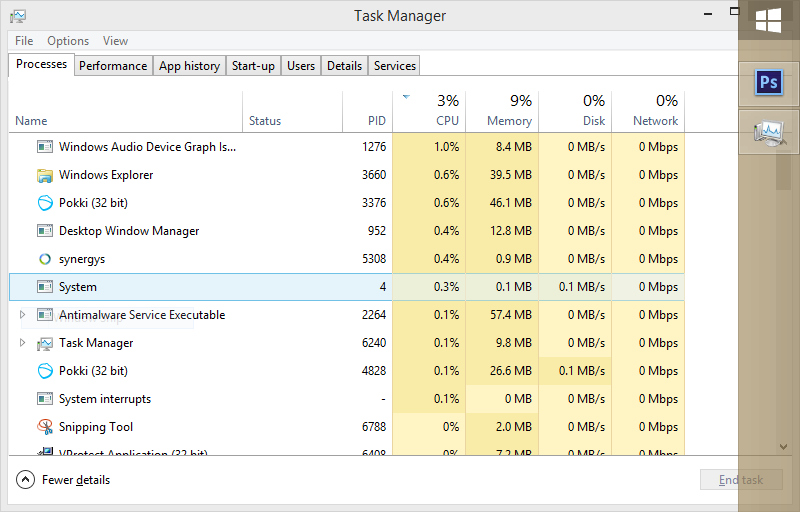
\includegraphics[width=200px]{images/Windows_Program_Manager_Screenshot}
  \caption{Windows Program Manager Interface}
  \label{fig:WinProcManScreen}
\end{minipage}%
\begin{minipage}{.5\textwidth}
  \centering
  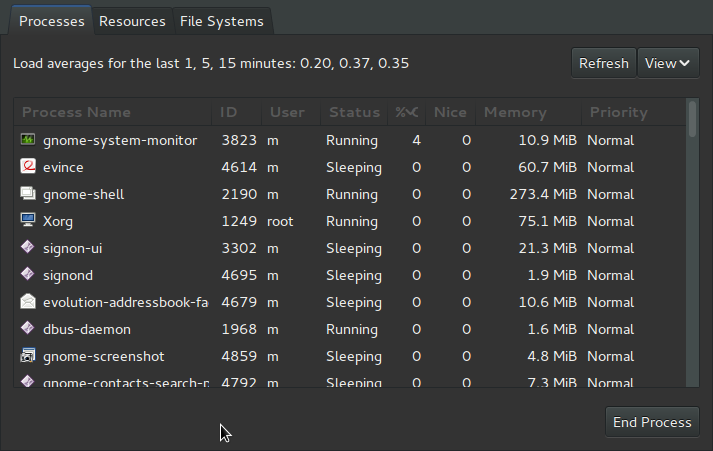
\includegraphics[width=200px]{images/Linux_Program_Manager_Screenshot}
  \caption{Linux Program Manager Interface}
  \label{fig:LinProcManScreen}
\end{minipage}
\end{figure}


\subsection{Using programs in Linux and Windows}

Interacting with programs is what users spend the majority of their time on a computer doing, because of this, it is a pivotal design aspect in modern Operating Systems. Some systems can be very different in how they allow you to interact with programs. Although the two reference systems were similar in how they present the programs to you, they differed when it came to navigating between programs.

In both the reference systems, the programs were presented in `floating', overlapping windows. These windows share the screen space by having the `active' window draw on top of all other windows. The system provides a way or moving, hiding, and resizing the windows to customize your workspace. Both systems provide similar mechanics for achieving this. They each provide a `title bar' that can be grabbed and dragged around to move the window. Each also provide the ability to grab the very edge of any side of any window, or the corners, to resize the window to the desired size. Finally, each system provides buttons to manipulate the windows more directly. This is where the systems begin to differ.

The Windows Operating System provides three buttons; The first Button allows the user to minimize the window to hide it from the work space. The second button is to maximize/un-maximize the window, this makes the window occupy the entirety of the screen. The final button exits the application.

The Linux Operating System only provides an exit button.

Figures \ref{fig:WinTitleBarScreen} and \ref{fig:LinTitleBarScreen} give example of these features.

\begin{figure}[ht]
\centering

\includegraphics[width=200px]{images/Windows_title_bar_screenshot}
\caption{Windows Title Bar Example}
\label{fig:WinTitleBarScreen}
\end{figure}

\begin{figure}[ht]
\centering

\includegraphics[width=200px]{images/Linux_title_bar_screenshot}
\caption{Linux Title Bar Example}
\label{fig:LinTitleBarScreen}
\end{figure}

Because of the nature of overlapping windows on both systems, it is possible for one window to be drawn entirely `under' another window. In Windows it is in fact possible to choose to hide a window from the workspace completely. In this situation the systems both provide different ways to navigate back to the `hidden' window.

On windows, There is a `task bar'. This is a portion of the screen, (often located at the bottom of the screen), that stores small icons for each running program. Clicking on one of these icons will bring that program to the front, un-minimize it, and make it the `active' program.

On Linux, Pressing the windows key, or pointing your mouse cursor to the corner of the screen shows you all of the open programs by `zooming out' and separating all the programs from each other. Selecting a program from this `exploded' view will un-minimize this window, bring it to the front, and make it the active window.

Figure \ref{fig:WinWinNavScreen} and \ref{fig:LinWinNavScreen} give example of these Navigation features.

\begin{figure}[ht]
\centering
\begin{minipage}{.5\textwidth}
  \centering
  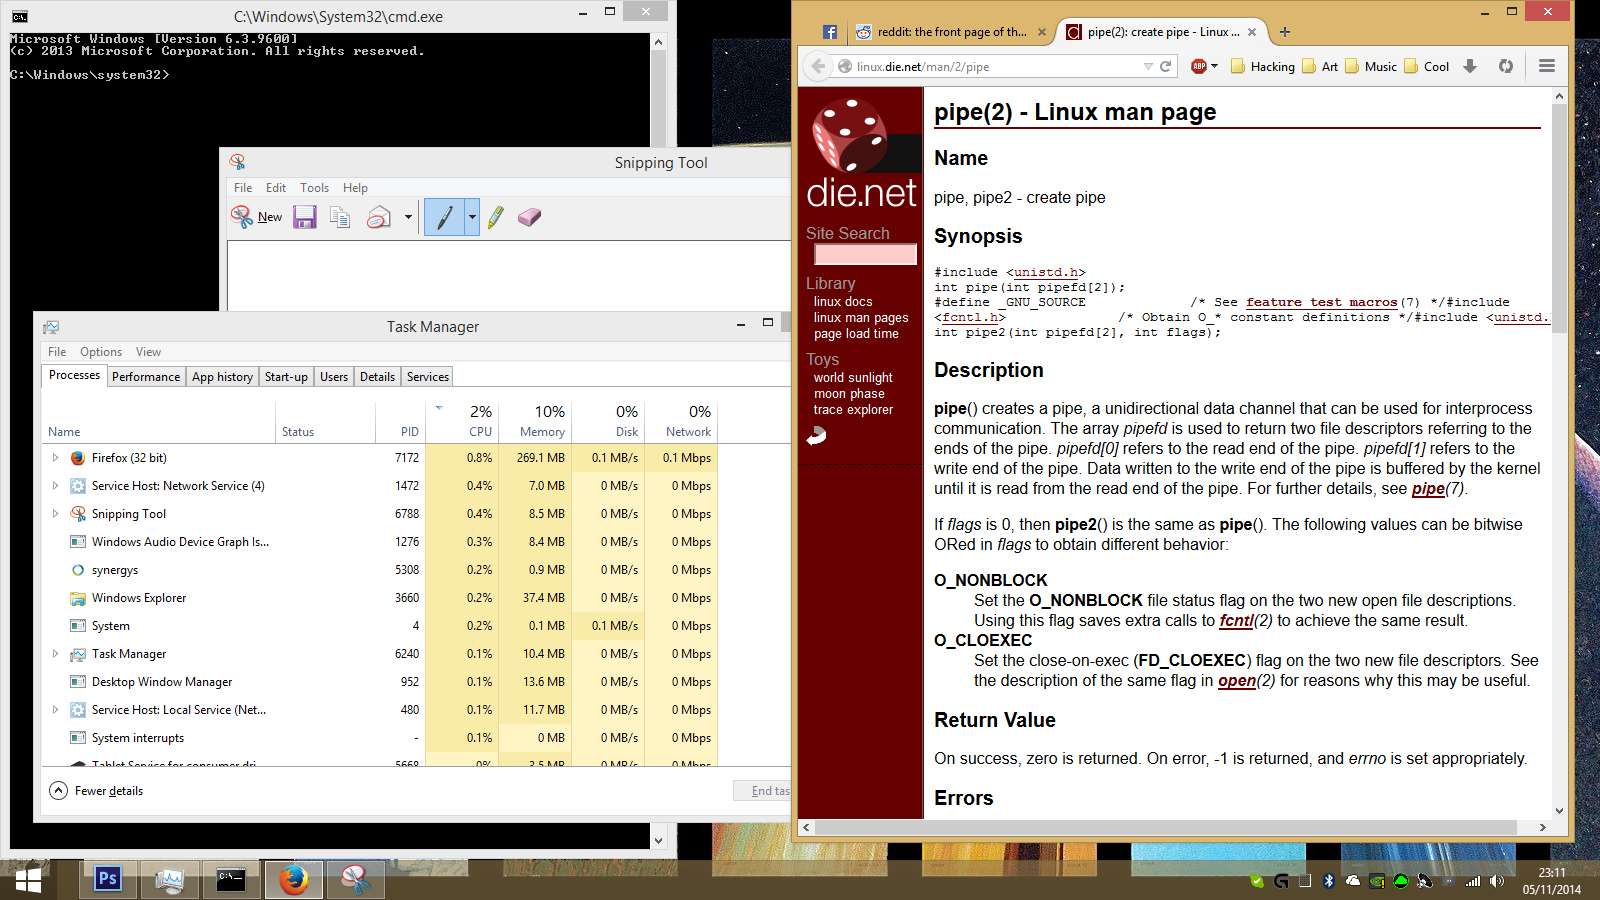
\includegraphics[width=200px]{images/Windows_Window_Navigation_Screenshot}
  \caption{Windows Program Navigation Interface}
  \label{fig:WinWinNavScreen}
\end{minipage}%
\begin{minipage}{.5\textwidth}
  \centering
  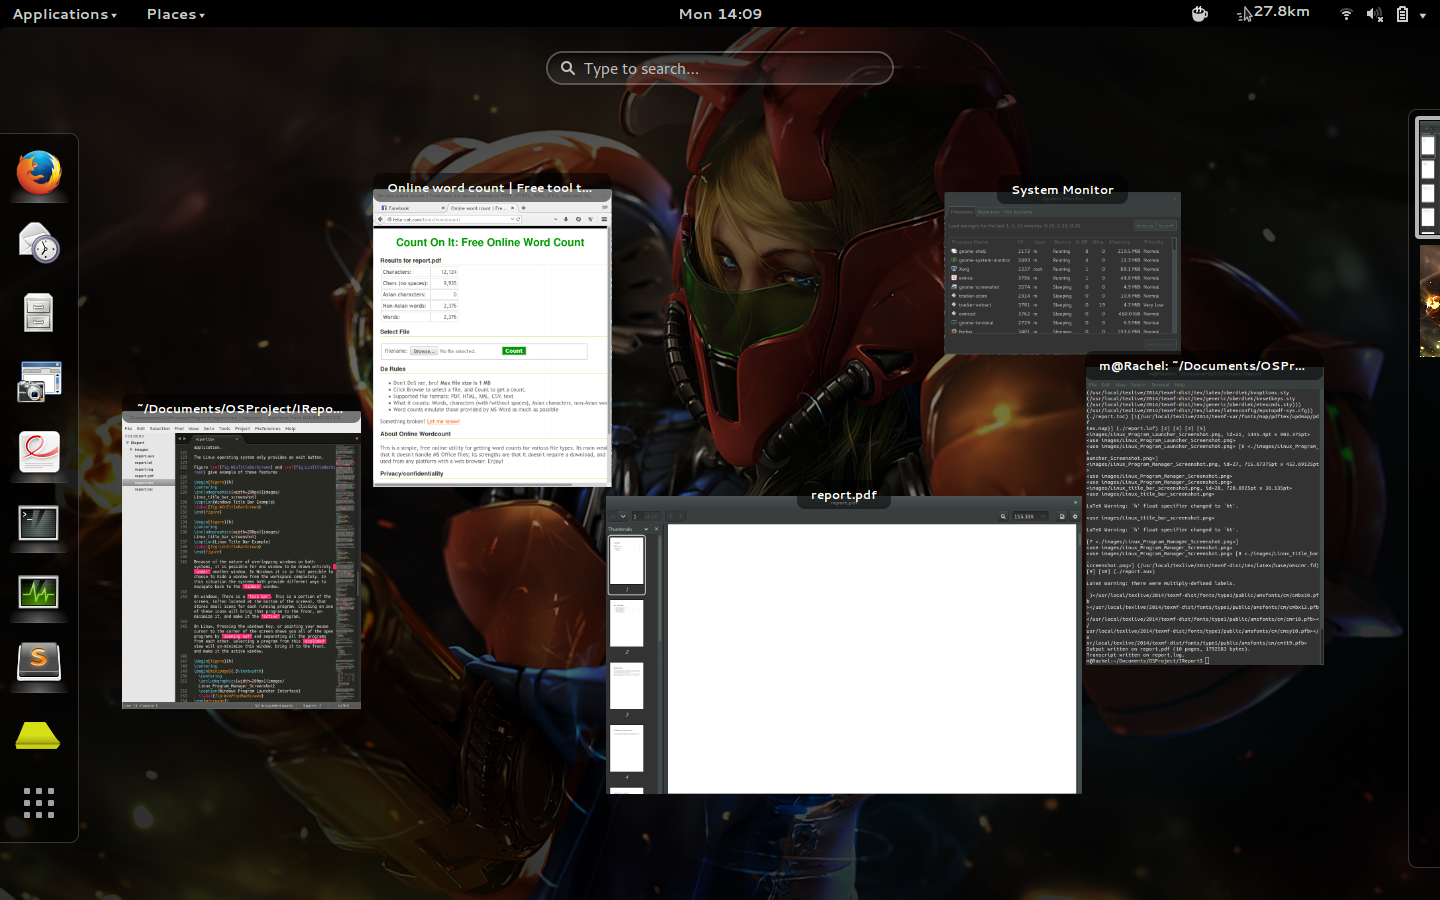
\includegraphics[width=200px]{images/Linux_Window_Navigation_Screenshot}
  \caption{Linux Program Navigation Interface}
  \label{fig:LinWinNavScreen}
\end{minipage}
\end{figure}


\clearpage
\section{The Program Developers}

To understand how program developers interact with Operating Systems The Linux distribution remix `Gnomebuntu' was studied. Only one system here was studied as Linux is an open source system. This meant that the system could be looked at in more depth.

The parts of the Linux system that were analysed are the; Process management system, the memory management system, the windowing system, and Inter Process Communication.

\subsection{Managing processes in Linux}

Linux exposes a number of system calls to the program developers to allow them to create, destroy, and pause processes, and also change the current `executable' to allow for new programs to be run.

\noindent
\textbf{Creating a new process}

To create a new process, Linux provide the `fork' system call. \cite{manFork}

Fork will spawn a new processes with a perfect copy of the calling processes memory and cpu state. This effectively means that fork will return twice, once into the caller and once into the child. It will return 0 to the child and the child pid to the parent.

\noindent
\textbf{Changing executable}

To change the executable that your process is running Linux provides execve. \cite{manExecve}

Execve will replace the calling processes memory with that of the target executable and then jump to the \_\_start label in the target executables code. This allows for switching into new executables and can be used along side fork to spawn new programs.

\noindent
\textbf{Destroying processes}

To destroy a process, Linux provides the `kill' system call. \cite{manKill}

In Linux, kill is not just for killing processes. It allows the caller to send a signal to the target process. Frequently the signal sent is SIGKILL or SIGTERM which both destroy the target processes in different ways.

\noindent
\textbf{Pausing and Restarting processes}

To pause and continue processes in Linux, the kill system call is re used, but now the caller sends the SIGSTOP signal.

\subsection{Managing memory in Linux}

Linux provides two functions for memory management, one to allocate memory and one to free it.

\noindent
\textbf{Allocating memory}

Linux provides the malloc call to allocate memory. \cite{manMalloc}

Malloc is passed the size of memory need in bytes and will return a pointer to the heap that is at least of the size requested.

\noindent
\textbf{Deallocate memory}

Linux provides the free call to deallocate memory.

Free is passed a pointer to memory that was received from malloc, it frees this memory allowing for it to be allocated during future calls to malloc.


\subsection{Managing screen space in Linux}

The screen space is not managed by the Linux kernel and so is not useful as a study for MOS.

\subsection{Inter Process Communication in Linux}

Communication between processes is an important part of creating complex behaviours in user space programs. Linux provides some simple calls to create channels of communication between processes.

\noindent
\textbf{Creating a pipe.}

Linux provides the `pipe' system call to create pipes. \cite{manPipe}

`pipe' created a one directional communication channel and provides the user a handle to this channel.

\noindent
\textbf{Reading and Writing to a pipe.}

To use this channel, Linux provides `write' and `read': \cite{manWrite} \cite{manRead}

These system calls will read and write using the pipe, allowing process to send data to each other. Note, it is by design that the pipe only transmits bytes, it is down to the user space program to define any communication protocols for transmitting more complex data.

\section{Analysis conclusion}

It was found that in end user design, many systems share similar design features. These features are very rich and operate do to a wide collection of tool, utilities, and applications The most important of these feature should be mimicked in new systems to assist new users in understanding how the the system works, However due to time constraints MOS will target much simpler versions of these features.

From the programmers perspective. The system API's or modern Operating Systems have been well thought out and have stood the test of time, however sometimes represent behaviours far more complex than that which MOS targets. The studied API's will be mimicked both to follow tried and tested ideas, and also so that program developers feel at home developing for MOS.

































\clearpage
\chapter{User Design}

As with the Analysis, the Design phase was separated into End User and Program Developer sections. The designs presented here are the final designs for the system, some earlier versions can be found in XXXXX.

Design for the end user focused on similar tools, looks, and controls to existing systems; The Linux CLI was referenced for a lot of the simple command line tools as MOS' text mode graphics share a common interface to Linux terminals. MOS programs also targeted a clean workspace, avoiding unnecessary ascii drawing and focussing on delivering the service provided in a quick and clean manner.

Program Developer design was constructed with a 'many simple tools' structure. Each system call the standard library contained was made to perform one task, rather than bunching many tasks into one more complex call. This allows developers to maintain simple, intuitive control over their resources.

\clearpage
\section{The End User}

The End Users interaction directly with MOS will be limited, as the majority of their time will be spent interacting with the user space programs running on the system. Because of this, MOS will ship with a number of user space tools for managing the system

The following actions will be possible using the built in tools.
\begin{itemize}
\item Process Creation.
\item Process Management.
\item File/directory Creation.
\item File/directory Management.
\item File editing.
\end{itemize}

\subsection {Process Creations : MASH}

MASH will be MOS' built in shell. Using MASH, users can launch any other process.

MASH will support passing parameters to launched processes, and a persistent file history. It will be displayed to the user as a single line at the bottom of the screen, with a \> prompt where the user can enter their command.

Since MASH will cover Process Creation. All other actions that user can perform with build in tools are achieved through different built in programs. The user can use MASH to launch these programs passing any desired parameters.

\subsection{Process Management : processes}

The program called processes will serve as the users tool for killing processes.

The proposed design for this program is given by the following example screen.

{\ttfamily \small
  \begin{framed}
    \begin{verbatim}

      Running Programs:

        PID     | Name     | CPU Usage     | Memory Usage  | Status     |
        0       | init     |           0 % |         8 KB  | Paused     |
      > 1       | time     |           2 % |         2 KB  | Running    |
        2       | notes    |           1 % |        25 KB  | Running    |
        5       | pong     |          80 % |       102 KB  | Running    |
        12      | name     |           0 % |         1 KB  | Paused     |

     Press k to kill the current [>] process.

    \end{verbatim}
  \end{framed}
}

As shown, this tool will show the user information about each running processes and afford them the ability to kill these processes.

\subsection{File/Directory creation: mkdir and touch}

MOS will provide two programs for creating files and directories. touch will create empty files and mkdir will create directories. Both programs will operate in a similar way, taking an absolute path as their only parameter. Neither will create anything unless the parent directory of the wanted object exists, and the parameter is well formed (with a training / for directories).

\subsection{File/Directory Management: rm and mv}

For file and directory management MOS will provide two functions.

The first is rm. rm will try to delete the object at the obsolete path path passed as its only parameter. This path must be will formed and the object must exist however rm does not mind if the object is a file or directory and will delete either. If a directory is selected, all child nodes of that directory will be delete recursively.

The second is mv. mv will take two parameters, the first will be the path to an existing file system object (file or directory) and the second will be the path to an existing directory. mv will move the specified object (and all of its children in the case of a directory) into the target directory.

\subsection{File Editing: notes}

MOS' provides a simple multi-line text editor for editing text files. The program takes one parameter which is a path to the file you wish to edit. If the file does not exist notes will create it.

Notes supports common cursor key commands for navigating the cursor and saves when ctrl+s is presses.
\section{The Program Developers}

As program developers are very familiar with how to create programs for other systems, the API for the project system was designed to be very similar to that of the Linux kernel that was analysed.

\subsection{Managing processes}

MOS will provide a very similar set of system calls to Linux, however their behaviour may be simpler.

These features were considered independently of each other except for creating a new process and changing the current executable, as these calls are so commonly used together.

\textbf{Creating a new process}

Similar to Linux the process creation pattern MOS was designed to follow the `fork and exec' pattern. Therefore MOS provides two system calls:

`fork()' will return the child pid to both the parent and the child, allowing for the processes to distinguish themselves by comparing this value to the value of the `get\textunderscore pid()' system call. On failure it will return -1.

`exec(pid)' takes the integer value of the target program to be loaded. It does not return. On failure the current process will not continue.

\textbf{Destroying processes}

Unlike in Linux, where destroying, pausing, and restarting processes uses one system call, MOS will use three separate calls.

`kill(pid)' will kill the target process, freeing all its memory and removing it from the scheduler.

\textbf{Pausing and Restarting programs}

Pausing programs is important for efficiency, therefore MOS provides the following calls.

`pause()' and `pause(pid)' will pause the target process until `wake()' is called. With `pause()' the current process will be paused and immediately revoke controls to the scheduler.

`wake(pid)' will wake the target process and allow it to be scheduled again. It will NOT cause the target process to be executed next.

\subsection{Managing memory}

The memory managemnt API will be Identical to that of Linux. Therefore MOS will provide two system calls:

`malloc(size)' will allocate a memory locations of size, and return a pointer to that location.

`free(pointer)' will deallocate the memory at a pointer.

\subsection{Managing screen space}

As the Linux screen management system cannot be mimicked in the MOS, a new one entirely was invented. This lead to one system call:

`setio(px,py,wx,wy)' will attempt to allocate the portion of the screen using the starting coordinate (px,py) and the size (wx,wy). If this failed (that portion of the screen is already allocated) the call will block. Otherwise it will reserve this portion of the screen for this process.


\subsection{Inter Process Communication}

The Interprocess Communication process will be very similar to Linux's system with one key addition.

`pipe(size, \&readpipe, \&writepipe)' will set up a communication channel of the requested size. On failure it will return one of a number of errors: -1 will indicate that the pipe cannot be created due to a lack of space, -2 will indicate that the system pipe table is full. This call will fill readpipe and writepipe with descriptors that can be passed to all the other pipe calls.

Once a pipe is set up three calls will be able to interact with it:

`write(pipe, byte)' will write the byte into the pipe. On failure it will return an error message; 1 will mean the pipe is full and 2 will mean the pipe is of the wrong type (a read-pipe not a write-pipe).

`read(pipe)' will return a positive byte representing the byte at the front of the pipe, or a negative error message; -1 will mean the pipe is empty and -2 will mean the pipe is of the wrong type.

`waitToRead(pipe)' will return a positive byte representing the byte at the front of the pipe or a negative error message; -2 will mean the pipe is of the wrong type. Note, if the pipe is empty, this call will block the process until the pipe is written to.

\chapter{Project Plan}

This project constitutes a significant amount of work, some of which is of undefined difficulty (it will be impossible to predict ahead of time how much time it will take to complete). However there is also a significant amount of time to complete it, if time is managed properly and work effort is consistent.

Because of this, an FDD (feature driven development) style of project management was chosen.

This style is where a feature that can be completed (all prerequisite features are complete) is selected, analysed, designed and then implemented. Once it is completed and tested, the process is repeated.

This style keeps project engineers focused on similar tasks, and prevents them from bouncing around tasks left, right, and center.

The FDD style requires that project engineers have a set schedule and during scheduled work hours focus on the task at hand.

The downside of an FDD project is it is difficult to get an estimate of when the project will be completed. However this does not matter so much as FDD is more concerned about quality progress over superficial deadlines.

The Project engineer has proposed this schedule for the project work (Figure includes non-project work hours to demonstrate correct time allocations.):


\begin{figure}[ht]
\centering
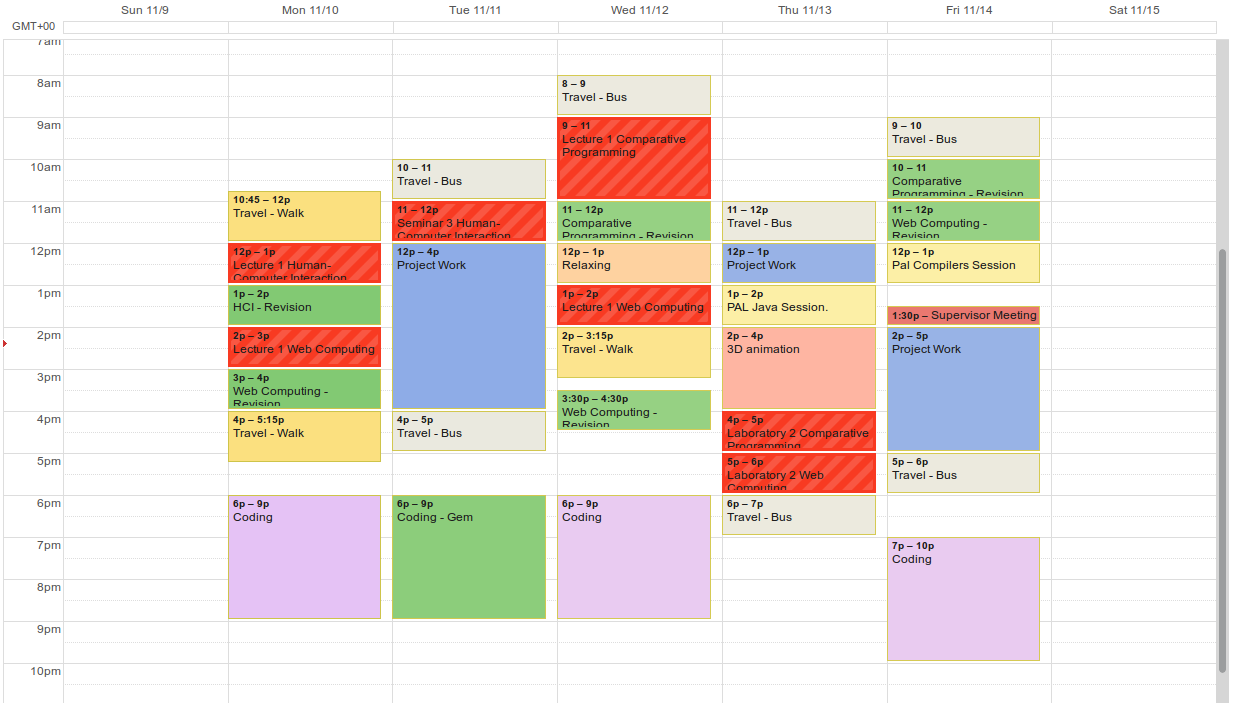
\includegraphics[width=450px]{images/schedule_screenshot}
\caption{Weekly Schedule. Project work shown in Blue, Extra project time shown in Purple.}
\label{fig:schedulerscreen}
\end{figure}


\chapter{Log}


\section{Week 1}
\begin{itemize}
\item Created basic design docs.
\item Rewrite existing code to be suitable for this project.
\end{itemize}

\section{Week 2}
\begin{itemize}
\item Detect Upper Memory.
\item Test Stack Jumping.
\item Simple page frame allocator.
\item Bound all interrupts to stubs.
\item Created simple kernel threading.
\item Created a `printf' like utility.
\item Supervisor Meeting 1: This week we discussed the state of the project, some goals to hit in the upcoming weeks and the proposal report due in next week.
\end{itemize}

\section{Week 3}
\begin{itemize}
\item Implemented Paging.
\item Moved to a higher half kernel.
\item Loaded my first `user space' program.
\item Supervisor Meeting 2: This week we discussed how process creation was handled in linux and other Operating Systems, and how to move forward with concurrency.
\end{itemize}

\section{Week 4}
\begin{itemize}
\item implemented fork system call.
\item implemented exec system call.
\item Supervisor Meeting 3: This week we discussed how IPC was handled on many different system and how I could think about going ahead with IPC.
\end{itemize}

\section{Week 5}
\begin{itemize}
\item major bug fixing.
\end{itemize}

\section{Week 6}
\begin{itemize}
\item created proposal for IPC.
\item implemented IPC.
\item began work on interim report.
\item Supervisor Meeting 4: This week we discussed how to continue work on IPC and the next steps of using the IPC to abstract general process I/O.
\end{itemize}

\section{Week 7}
\begin{itemize}
\item finished work on interim report.
\end{itemize}

\chapter{Appendices}

The following Three pages are a copy of the Project Proposal document.

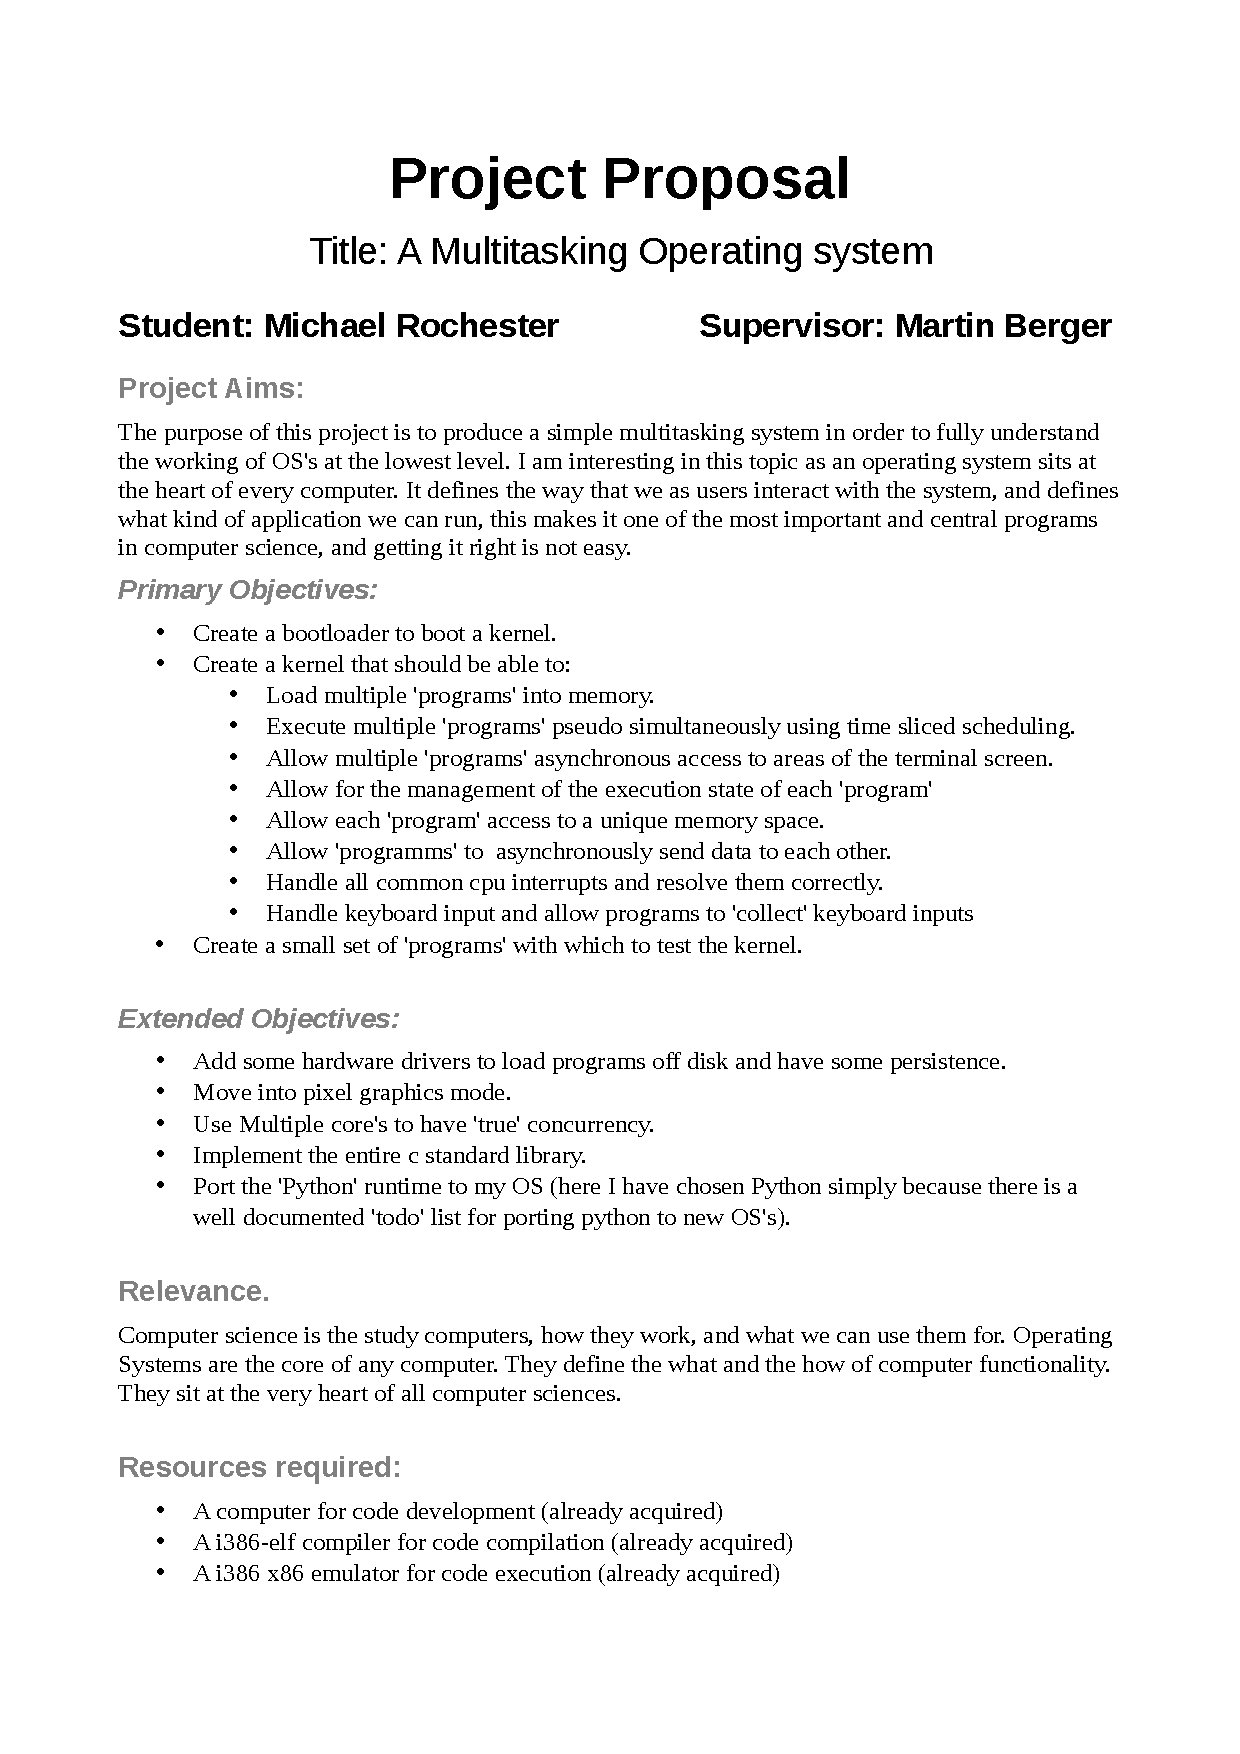
\includepdf[pages=-]{images/proposal_doc}




\bibliography{report}
\bibliographystyle{unsrt}

\end{document}